\section{Prozesse}
\textbf{Monoprogrammierung: }2 SW-Akteure (OS, Programm), Programm kennt nur OS \& sich selbst (ist isoliert)
\textbf{Quasi-Parallel: }Programme gleichzeitig in Hauptspeicher, Ausführung nacheinander, für Isolation: jeder Prozess virtueller Adressraum
\textbf{Prozess umfasst: }Abbild des Programms (text section), globale Var. (data section), Speicher für Heap (startet bei kleinster Nr.)$\leftrightarrow$Stack (startet bei grösster) \textbf{Eigenschaften Prozess: }eigener Adressraum, frei Registerbelegung, Isolation (gut für unabhängige Appl.) \textcolor{red}{-} gemeinsame Ressourcen schwierig, grosser Overhead für Prozesserzeugung, Realisierung Parallelisierung aufwändig
\subsection{Process Control Block (PCB)}
OS benötigt Daten für Integration des Prozesses im Gesamtsystem, PCB eines Prozesses beinhaltet: Eigene ID, Parent ID andere wichtige IDs | Speicher Zustand Prozessor | Scheduling-Infos | Daten für Sync/Kommunikation zwischen Prozessen | Filesystem-Infos | Security-Infos

\subsection{Interrupts}
Auftreten eines Interrupts, Ablauf:
\begin{enumerate}
    \item context safe: Register, Flags, Instruction Pointer, MMU-Config(Page-Table-Pointer)
    \item Aufruf Interrupt-Handler, kann Kontext überschreiben
    \item context restore: Wiederherstellung des Prozesses aus PCB
\end{enumerate}
Kontext-Wechsel sehr teuer (viele Register inv.), Cache hier als Nachteil$\rightarrow$alles muss gewechselt werden

%\subsection{Erzeugen eines Prozesses}
%Aus Programm Prozess machen: 1. Prozess erzeugen 2. Image des Programms in Prozess laden \& in laufbereiten Zustand versetzen

\subsection{Prozesshierarchie}
Tool: \prgc{pstree}, jeder Prozess: 1 Parent-Prozess, beliebige Anz. Child-Prozesse | sytemd (PID 1): init Prozess$\rightarrow$Starten, Beenden \& Überwachen von Prozessen

\subsection{API}
exakte Kopie des Prozesses, ausser: Child hat eigene/andere Prozess-ID
\begin{minted}{c}
pid_t pid = fork();//Rücksprung beide
if (pid > 0){/*Parent Code*/}
else if (pid == 0){/*Child Code*/}
//-1 Fehler, errno
\end{minted}
\prgc{pid_t wait (int * status)} unterbricht Prozess bis 1 Child-Prozess beendet | \prgc{status} Out-Parameter, Abfrage durch Makros\\
\prgc{pid_t waitpid (pid_t pid, int * status, int options)} \\
\prgc{pid == -1} auf irgendein Child-Prozess, wie \prgc{wait()}\\

gerade laufender Prozess: Programmimage ersetzt durch anderes 
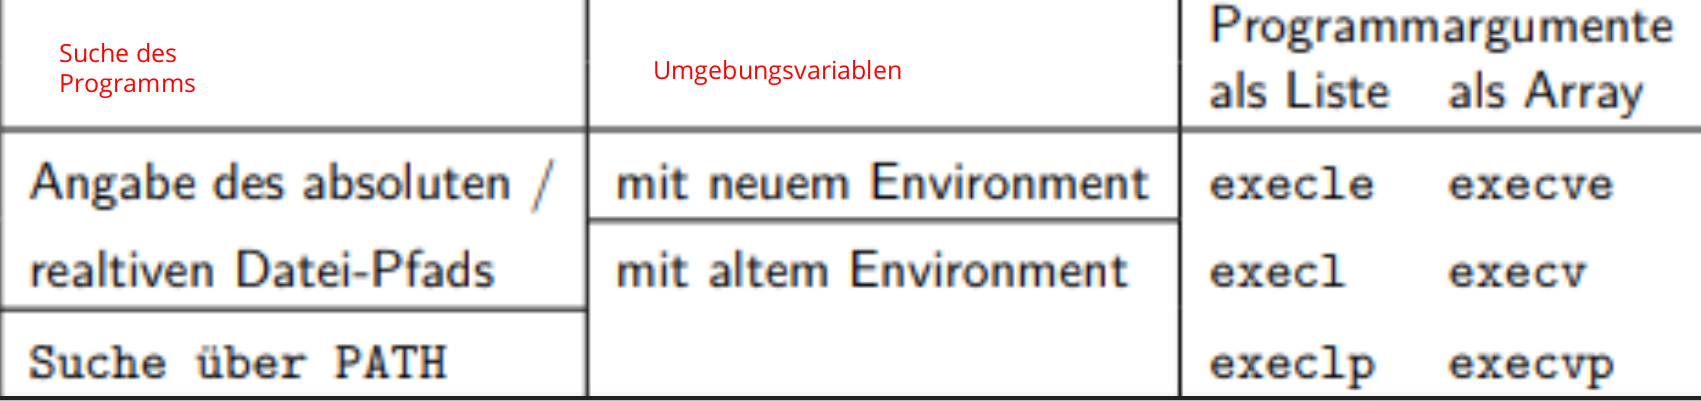
\includegraphics[scale = 0.1]{grafiken/exec.png}

\prgc{unsigned int sleep (unsigned int seconds)}\\ 
durch Signale unterbrochen, Anz. verbleibende Sek. zurück\\

\prgc{void exit (int code)}\\
\prgc{int atexit(void (*function)(void))}\\
Aufräumfunktion mitgeben, in umgekehrter Reihenfolge nach Exit ausgeführt 

\prgc{pid_t getpid(void)}, \prgc{pid_t getppid(void)}

\subsubsection{Zombieprozess}
Child zwischen seinem Ende und Aufruf von \prgc{wait()} Zombie\\
Parent verantwortlich, OS behält Statusinfos bis zum Aufruf
\textbf{Dauerhafter Zombie: } Parent ruft wait nicht auf (vermutlich Fehler), Lösung: Parent stoppen $\rightarrow$ Childs werden zu Orphants

\subsubsection{Orphanprozess}
Parent Prozess beendet $\rightarrow$ alle Child-Prozesse verwaisen, werden an Prozess Nr. 1 übergeben
systemd: ruft wait in Endlosschleife auf